%%%%%%%%%%%%%%%%%%%%%%%%%%%%%%%%%%%%%%%%%
% University Assignment Title Page 
% LaTeX Template
% Version 1.0 (27/12/12)
%
% This template has been downloaded from:
% http://www.LaTeXTemplates.com
%
% Original author:
% WikiBooks (http://en.wikibooks.org/wiki/LaTeX/Title_Creation)
%
% License:
% CC BY-NC-SA 3.0 (http://creativecommons.org/licenses/by-nc-sa/3.0/)
% 
% Modified for COSC480/490 by:
% Lech Szymanski (8/3/18)

\documentclass[12pt]{article}
\usepackage[draft]{cosc4x0style}
\usepackage{biblatex}
\usepackage{listings}
\usepackage{verbatim}
\addbibresource{refs.bib}

% To compile the final version of the report (which will remove all the todo content)
%\usepackage{cosc4x0style}

% Specify project code 480 or 490
\papercode{480}

% Your project title
\title{An Exploration of the Common Vulnerability Scoring System}

% Your name
\author{Jake \textsc{Norton}}
\studentid{5695756}

% Names of your supervisors, separated by line break '\\'
\supervisors{
  Dr. David \textsc{Eyers} \\
  Dr. Veronica \textsc{Liesaputra}
}

% Date, change the \today to a set date if you want to be precise
\reportdate{\today}

\begin{document}


\maketitle

\begin{abstract}

	The Common Vulnerability Scoring System(CVSS\cite{CVSS}) is designed to produce scores for
	software vulnerabilities. Such a system is needed in order to triage the sheer number of new
	vulnerabilities being released every year. We cannot keep up with the amount of CVSS scores that
	need to be produced, as such we need a way to generate them. There is precedent to using machine
	learning, specifically in more recent times, large language models(LLMS) to accurately predict
	these CVSS scores.\cite{costa} However, there is a general focus on only using the National
	Vulnerability Database\cite{costa}\cite{nvd_example1}\cite{nvd_example2}, it would be ideal if
	there was more than one source for the ratings, not only for cross validation, but also for an
	increase in data. Before we use any extra data sources, it will be interesting to do a
	comparison between the different sources, to see if we can get an estimate accuracy for each of
	the metrics within the scoring system. Additionally we should know how good of a system CVSS is
	and whether or not there are better alternatives. Unfortunately CVSS(version 3.1\cite{CVSS_31}) is a flawed
	metric, hopefully once 4.0 begins to be used commonly that will solve some of these issues.
	However, the ability to predict a metric based on a short text description is still useful and a
	focus on the interpretability of such a system remains important.

\end{abstract}

\begin{figure}
	\centering
	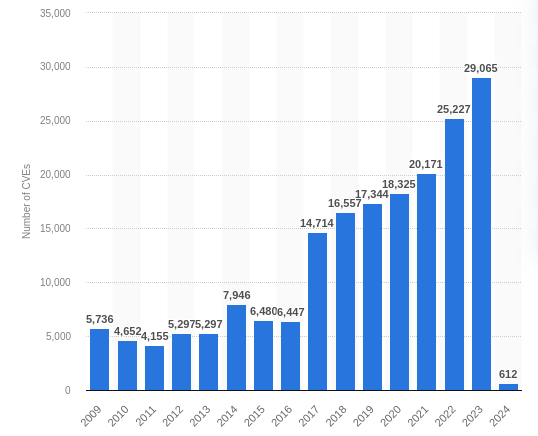
\includegraphics[width=0.5\textwidth]{figures/cve_year.png}
	\caption{\label{fig:cve_year}Number of new CVEs by year}
\end{figure}

\section{Introduction}

Last year there were 29,065 new vulnerabilities. This is a number that is only going up year on
year. Now, we need a way to record these vulnerabilities, and we do that using the common
vulnerabilities and exposure system called CVEs. From these CVEs, CVSS scores can be calculated or
generated. The National Vulnerability Database(NVD\cite{NVD}) takes the CVEs and enriches them with
CVSS data. They are not the only place to do so, however in terms of research they are often the
main or sole data provider.\cite{costa}\cite{nvd_example1}\cite{nvd_example2} I explored other
options, the main obvious one being the MITRE\cite{MITRE} database, as it is the main database for
CVEs and they also have a decent chunk of CVEs enriched with CVSS scores. As a guideline to my
investigation between the two databases I used the same method as the paper \textit{Can the Common
	Vulnerability Scoring System be Trusted? A Bayesian Analysis}.\cite{bayes} This paper tries to see
how much different data sources agree on the scoring of a CVE, and thereby gaining insight into the
potential of a ground truth value. Unfortunately since that paper in 2016, many of the databases
they compared are either unavailable or in archival status. However, following their method still
allows for insight between the two chosen databases, NVD and MITRE. This analysis shows that the
databases do fundamentally rate CVEs differently. The uncertainty between the two can therefore be
an indicator going forward when analysing generated CVE scores, as it is likely that the model will
also struggle in similar places to where the human evaluators did. In addition to this analysis, I
looked into the CVSS system itself. There have been many complaints laid against
CVSS\cite{ubiquitous}\cite{improving_cvss}\cite{time_to_change_cvss}, the main ideas being:

\begin{itemize}
	\item Mathmatical operations on categorical values,
	\item No mathmatical basis for the formula,
	\item Lack of likelihood,
	\item Scope has too much influence,
	\item Identity crisis,
\end{itemize}

These are all on going issues and should colour how we use the CVSS system. It should only be used as a way to triage our vulnerabilities, any further
prioritisation should be done by more specific inqueries or perhaps other systems.

\section{Background}

Vulnerabilities are stored in a consistent system called Common Vulnerabilities and
Exposures(CVE\cite{CVE}).

\subsubsection*{Here is an example CVE}
\begin{itemize}
	\item   Unique Identifier: CVE-2024-38526
	\item   Source: GitHub, Inc.
	\item   Published:06/25/2024
	\item   Updated:06/26/2024

	\item   Description: pdoc provides API Documentation for Python Projects. Documentation
	      generated with `pdoc --math` linked to JavaScript files from polyfill.io. The polyfill.io
	      CDN has been sold and now serves malicious code. This issue has been fixed in pdoc 14.5.1.

\end{itemize}

\footnotesize{Sourced from \href{https://nvd.nist.gov/vuln/detail/CVE-2024-38526}{NVD CVE-2024-38526
		Detail}\cite{polyfill}} \\
\bigskip

This has a unique identifier, which is given by one of the CVE numbering authorities(CNA\cite{CNA}), such as
GitHub, Google and many other
organizations.[\href{https://www.cve.org/PartnerInformation/ListofPartners}{CVE list of
			partners}\cite{partners}]
The description is the most important part in our case. This should give some information about the
vulnerability, what can be exploited (device / software component), how is the product affected if
the vulnerability is exploited. In this case we have the library PyDoc and this links to the
polyfill.io CDN. Ideally there would be something in the description which relates to every metric,
unfortunately these descriptions are not necessarily suited to machine learning as the people
writing the descriptions are expecting a lot of intrinsic knowledge.

\subsection*{The Common Vulnerability Scoring System}

CVSS scoring is a high level way to break up vulnerabilities into different categories.
Organisations can use it to choose which vulnerability to focus on first. CVSS is broken up into 3
distinct sections, base, temporal and environmental scores.

For brevity I will only show the specifics of CVSS 3.1\cite{CVSS_31}as this is by far the most commonly used
version, even if it is not the most recent.

\subsubsection*{Base Score}

\begin{itemize}

	\item Attack Vector: Defines the avenues of attack that the vulnerability is open to. The more
	      open a component is, the higher the score. This can have the values Network, Adjacent, Local
	      and Physical.

	\item Attack Complexity: How complex the attack is to orchestrate. What are their prerequisites,
	      how much domain knowledge / background work is necessary, how much effort does the attacker
	      need to invest to succeed. This can have the values Low or High. Low gives a higher base
	      score.

	\item Priviledges Required: The degree of privileges the user needs to complete the attack.
	      Generally ranging from None, Low(e.g User level privilege), High(e.g Administrator). The
	      lower the privilege the higher the base score.

	\item User Interaction: If the exploit requires another human user to make the attack possible,
	      E.g clicking a phishing link. This is either None or Required, the score is highest when no
	      user interaction is required.

	\item Scope: Defines if the attack can leak into other security scopes. E.g access to one
	      machine gives the ability to elevate privileges on other parts of the system. This can take
	      Unchanged or Changed, the score being highest when a scope change occurs.

	\item Confidentiality Impact: Detemines what is the impact on the information access /
	      disclosure to the attacker. This can be High, Low or None with High adding the most to the
	      base score.

	\item Integrity Impact: Refers to the integrity of the information within the component. I.e
	      could the data have been modified by the attacker. This has High, Low or None as categories
	      with High adding the most to the base score.

	\item Availability Impact: Refers to the impact of the attack on the availability of the
	      component. E.g the attacker taking the component off the network, denying the users access.
	      This can haved High, Low and None with High adding the most to the base score.

\end{itemize}

\footnotesize{This is a summarized version of the
	\href{https://www.first.org/cvss/v3.1/specification-document}{3.1 specification document
		provided by FIRST}.\cite{CVSS_31}}


\subsubsection*{Temporal}


\bigskip

This could be:
\begin{itemize}

	\item Exploit Code Maturity: The state of the attack itself, e.g has this exploit been pulled off in the wild or is it currently academic.

	\item Remidiation Level: Broadly, whether the exploit in question has been patched,

	\item Report Confidence: The degree of confidence in the CVE report itself, the report may be in early stages where not all of the
	      information is known.

\end{itemize}
\
\footnotesize{This is a summarized version of the
	\href{https://www.first.org/cvss/v3.1/specification-document}{3.1 specification document
		provided by FIRST}.\cite{CVSS_31}} \\
\bigskip

Temporal metrics would be useful in general for a CVSS score, however NVD do not store these
temporal metrics. As far as I can tell there is no reason given for this specifically, though
discourse
\href{https://security.stackexchange.com/questions/270257/cvss-v3-and-v3-1-missing-temporal-metrics-exploit-code-maturity-and-remediation
}{(Stack exchange post)}\cite{stack_exchange} around the subject suggests that this is due to a lack
of verifiable reporting. From my perspective both remidiation level and report confidence feel like
they could have scores attributed to them, however finding verifiable reports on the exploits seen
in the wild does seem more tricky. There are two relatively new organisations on this front,
Cybersecurity \& Infrastructure Security Agency(CISA,
\href{https://www.cisa.gov/known-exploited-vulnerabilities-catalog}{public sector}) and
inthewild.org(\href{https://inthewild.io/}{private sector}\cite{cisa}).

\subsection{Data Options}

In 2016 when Johnson et al\cite{bayes} did the original paper, they had access to 5 different
databases. Unfortunately only 2 of these remain for modern data, there are some others, but
essentially they are either in archival status or they are proprietary. I have managed to acquire
the data from the original paper, however it is in a much different format(XML vs JSON), and Pontus
Langstrom, one of the contributors to the project said it would be akin to an archaeological dig.
Additionally as I did not plan to make this the full focus of the project, that will sit dormant for
now.

\subsubsection*{National Vulnerability Database}

The National Vulnerability Database is the defacto standard dataset used for CVSS generation
research.\cite{costa}\cite{nvd_example1}\cite{nvd_example2} This makes a lot of sense as it is built
for the purpose with a team dedicated to enriching CVEs with CVSS scores. The dataset I am using was
retrieved using the NVD API in March 2024 and contains $\sim$100000 CVEs enriched with CVSS scores. This
comes in a easy to use format, in a consistently formatted JSON dump.

\subsubsection*{MITRE Database}

MITRE is the defacto database for the storage of CVEs themselves, however they do contain $\sim$40000
CVEs enriched with CVSS 3.1 scores. These are also in a JSON dump retrieved also in March 2024. The
format for usage is a bit more cumbersome to use. The CVSS scores are only stored as CVSS vector
strings(a simple text encoding\cite{vector_string}). These are not hard to parse, though they are stored slightly
different between versions, as well as sometimes being inconsistent($\sim$5000 had temporal metrics within
the vector strings in the MITRE database).

\subsubsection{Priliminary Data exploration}

The scorers for both NVD and MITRE do rate CVEs reasonably similar, one pattern you can see as shown
by Fig~\ref{fig:counts}, is that NVD generally give the most common categorical output more ratings.
They are less spread out across the full range of values. In addition, if we look at the
attackComplexity metric, there is a reasonably large difference in how they are rated, MITRE rate a
lot more of the metrics with a low score. This points to some of the difficulty with this kind of
rating system, while in theory there is a true value for these metrics, it requires knowledge of the
whole space around each of the vulnerabilities, this knowledge will always vary marker to marker.


\begin{figure}
	\centering
	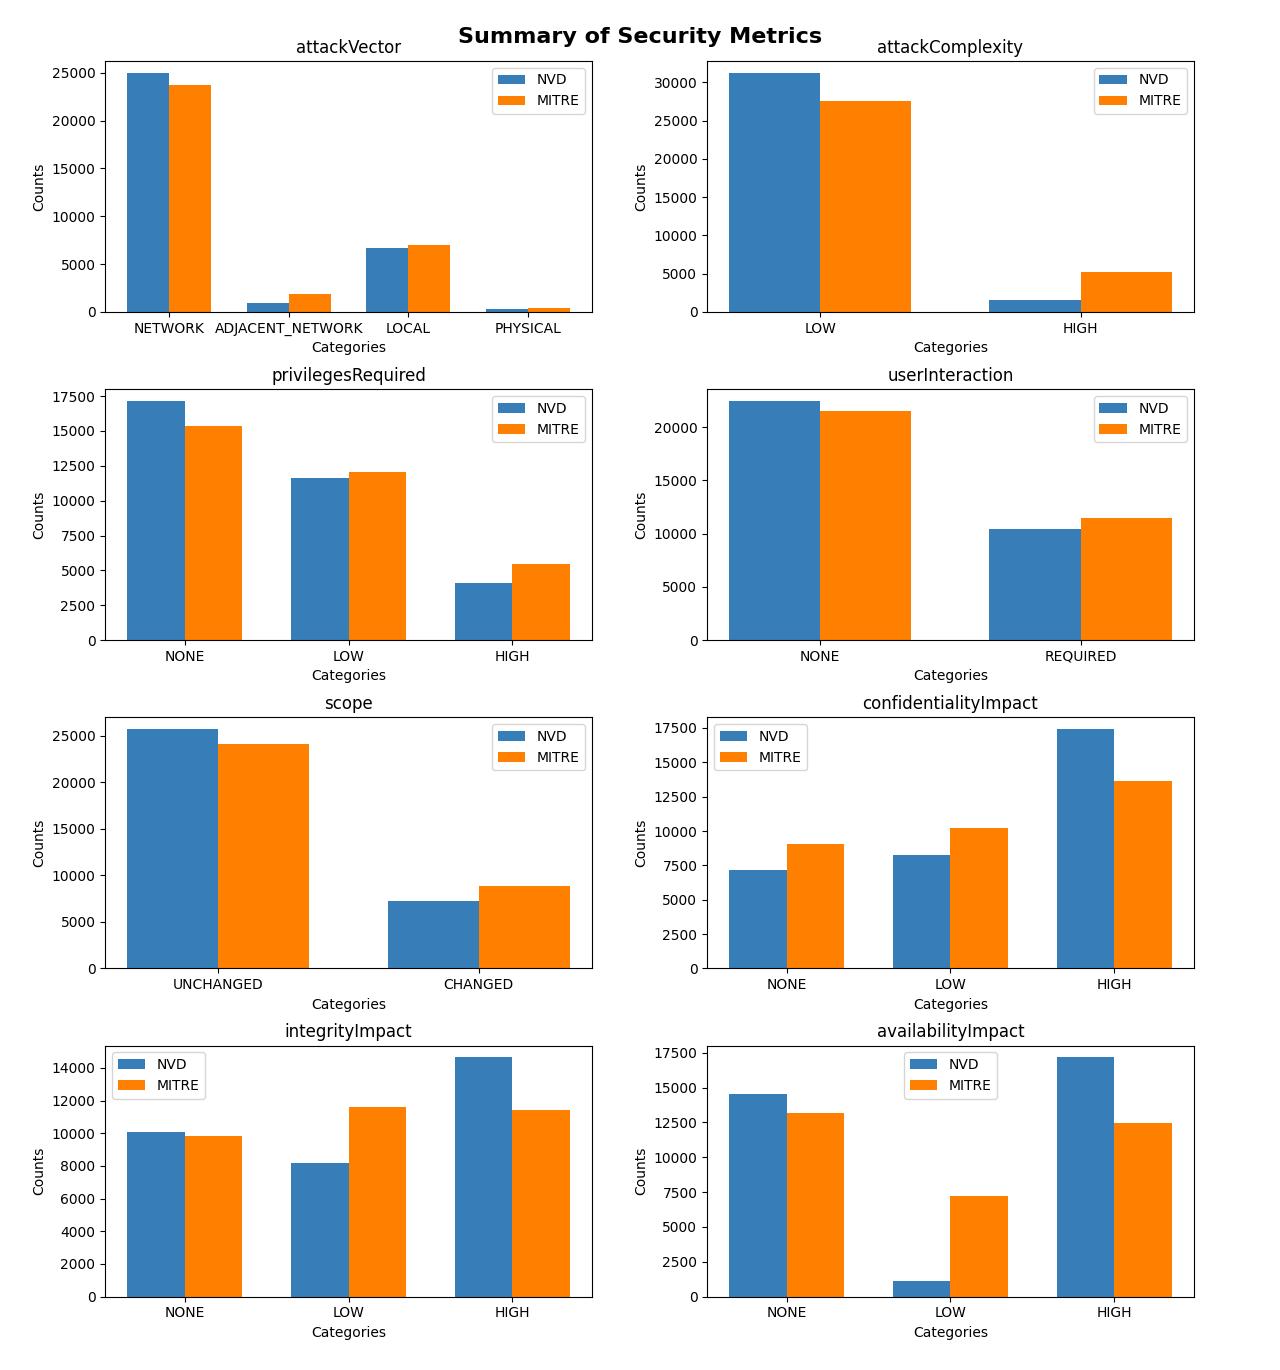
\includegraphics[width=1\textwidth]{figures/combined_overlap.png}
	\caption{\label{fig:counts}Comparison of CVSS ratings between MITRE and NVD}
\end{figure}

\section{Methods}

\subsection{Hierarchical Bayesian Model}

The analysis between the two databases is done with a hierarchical bayesian model. This type of
model is suitable when you expect the population to be similar in some respects but different in
others. In this case they share common knowledge towards the vulnerability mostly, but differ the
experience of the people rating the metrics.\cite{bayes} The model is similar to the original
model(see section 4.1 of \cite{bayes}), it assumes that there exists a true value for each CVSS
dimension, but the database sample may not be that true value. We represent the inaccuracies with a
confusion matrix. The A difference from the original paper is that there is no longer consistently 3
variables for each CVSS metric, varying from 2 to 4 categorical choices. \\

\bigskip

The confusion matrix CVSS dimension \textit{confidentiality impact}


\begin{equation}
	\Pi_ci = \begin{bmatrix}
		\pi_{nn} & \pi_{nl} & \pi_{nh} \\
		\pi_{ln} & \pi_{ll} & \pi_{lh} \\
		\pi_{hn} & \pi_{lh} & \pi_{hh} \\
	\end{bmatrix}
\end{equation}
where $\pi_{nn}$ denotes the probability that the current database correctly assigns the random
vulnerability \emph{none} when the actual value is the same. $\pi_{nl}$ and $\pi_{nh}$ represent
when \emph{none} was not the actual truth value.

\subsubsection{Priors}

The priors for the categorical variables were set up with uninformative priors using a Dirichlet
distribution, this will give a uniform prior over they probability space for all categorical
options. This is done to not colour the outcome of the results based on prior belief, but either
way this prior will have little impact for any categorical metric which has more than the number of
options for that metric.

The confusion matrices also need priors, for this they will also be a Dirichlet distribution,
however as we do want to add some initial belief to this, in that the people producing scores are
not acting completely randomly, and are likely to be right more often. These are still weak priors
as the number of observations is in the thousands.

\subsubsection{Estimation}

This follows, the Bayesian approach, where to estimate the parameters, you take the prior beliefs,
take an observation, and update these believes to produce posterior beliefs. In this case the method
involves using Markov Chain Monte Carlo methods. Broadly this allows for simulating the data based
on the previously created distribution by sampling values that the model has high belief would be
from the target distribution. This allows for accurate sampling without having all of the data. The
original paper used JAGS\cite{JAGS} and R. As I am more familiar with python I did try
pyjags\cite{pyjags} however I did not find great success. Instead I used the pymc library to help
with the modelling, it fulfilled the same tasks that JAGS did with the original paper\cite{bayes}

\subsection{CVSS Prediction}

Cody Airey--a classmate of mine-- has been working on a similar problem. He has been repoducing some
results from Costa et al.\cite{costa}. My choice of model for CVSS prediction will very much
bootstrap of his work and that which is surrounding it. So far, a strong contender for
state-of-the-art model for predicting CVSS metrics from CVE descriptions is the distilbert
model\cite{distilbert}. This is a variant of BERT\cite{BERT}, a pre-trained deep bidirectional
transformer large language model developed by Google. Distilbert has advantages over the models in
terms of performance, but also on speed of training as well as size / memory footprint of the
model.

\subsubsection{Training}

The model is trained separately for each metric. Following Airey's method, each of the eight models
were trained on five different data splits to allow for a standard deviation to be calculated, in
order to aid in reducing the chance of a 'good' data split effecting the results. The difference
between Costa et al. \& Airey's work and mine is that this model was trained on a combination of NVD and MITRE
data. This was converted to the same format, a CSV containing the descriptions and the CVSS scores.
This does mean there are now $\sim$40000 duplicate CVEs and $\sim$140000
\section{Discussion}

\subsection{Should we use CVSS?}
% \todo[inline]{Read https://theoryof.predictable.software/articles/a-closer-look-at-cvss-scores/}

CVSS has an identity crisis. Throughout its history, when originally released it was touted as a
solution to the task of prioritising CVE remediation as well as an assessment of risk, "IT
management must identify and assess vulnerabilities across many disparate hardware and software
platforms. They (IT management) need to prioritize these vulnerabilities and remediate those that
pose the greatest risk. The Common Vulnerability Scoring System (CVSS) is an open framework that
addresses this issue"

%[Peter Mell, Karen Scarfone, and Sasha Romanosky. 2007. The common vulnerability scoring system
%(CVSS) and its applicability to federal agency systems. Retrieved from
%https://www.govinfo.gov/content/pkg/GOVPUB-C13-19c8184048f013016412405161920394/pdf/]

However, due to a lot of feedback from the community and security agencies, when FIRST released
version 3.1, the authors state "CVSS Measures Severity Not Risk".

\subsubsection*{Severity vs Risk}

The severity ideally is a measure of the impact(worst case? Or different levels?). Risk is the
likelihood of the event happening. However in CVSS this is a bit muddied as even the Base score
includes some aspects which defaults to worst case risk.

Should use some way of temporal / environmental. These are included in CVSS however, they are often
not used and it may be better to use EPSS, which gives a numerical value of the likelihood of the
event happening in 30 days based on previous history

FIRST give this definition of severity vs risk
\textit{}
% CVSS Base scores (CVSS-B) represent "Technical Severity"
% Only takes into consideration the attributes of the vulnerability itself
% It is not recommended to use this alone to determine remediation priority

% Risk is often a religious topic… but…
% CVSS-BTE scores take into consideration the attributes of the…
% Base Score
% Threat associated with the vulnerability
% Environmental controls / Criticality 
% }

As mentioned by FIRST, the exact differences between risk and severity are strangely nebulous,
however here is a more usable definition as stated by NIST

"Risk is a measure of the extent to which an entity is threatened by a potential circumstance or event, and is
typically a function of: (i) the adverse impacts that would arise if the circumstance or event occurs; and (ii) the
likelihood of occurrence"
%NIST SP 800-30 Rev.1 Guide for Conducting Risk Assessments and the Committee on National Security
%Systems Information Assurance Glossary

There have been myriad complaints about this topic, generally due to the nature of how CVSS is often
used, especially in the US. There are many known occurences of the US government mandating the use
of CVSS base score as the primary framework used to prioritize remediation.


\printbibliography[title={References}]



% % Activate the appendix
% % from now on sections are numerated with capital letters
% \appendix

% \renewcommand{\thesection}{Appendix \Alph{section}}

% \section{Some extra things}

% If you have anything more to add such as:
% \begin{itemize}
% 	\item not essential details - things that might be too much for first time reading, or could be distracting from the main points...but are still important for reproducibility or deeper understanding
% 	\item work that was done in the project but doesn't go with the
% \end{itemize}

\section{Aims and Objectives}


\subsection*{Original}

\paragraph{Aims}
The primary aim of this research is to develop sophisticated predictive models capable of accurately determining
the severity levels of security threats based on the CVSS. This will involve a comprehensive review and comparison
of current datasets, with a focus on leveraging natural language descriptions provided in security vulnerability reports.
The project intends to utilize advanced transformer-based models to achieve this goal, contributing to the field of
cybersecurity by enhancing the precision of threat severity assessments.

\paragraph{Objectives}
\begin{itemize}[noitemsep]
	\item Conduct a comprehensive literature review to understand the current landscape of CVSS score prediction and the methodologies employed in existing models.
	\item Replicate successful methodologies to verify the accuracy of CVSS score databases, with a particular focus on alignment with recent CVSS standards and datasets.
	\item Explore opportunities for enhancing existing methodologies, including the investigation of data amalgamation from multiple databases to ascertain improvements in model performance.
	\item Experiment with various model architectures to identify the most effective approach in terms of predictive accuracy, specifically focusing on metrics such as the F1 score and balanced accuracy.
\end{itemize}

\paragraph{Timeline}
\begin{itemize}[noitemsep]
	\item March: Initiate the project with a literature review, system environment setup, and resource gathering.
	\item March-April: Replicate existing methodologies to validate findings and ensure alignment with current standards.
	\item May-June: Generate preliminary results and compile an interim report detailing findings and methodologies.
	\item July-August: Conduct experiments with various data source combinations and model architectures to identify optimal configurations.
	\item September-October: Finalize experimental work, analyze results, and prepare the comprehensive final report.
\end{itemize}

% \subsection*{Revised}

% \paragraph{Aims}
% Here you are describing the term goal of the project.  What do you want to achieve by the end?  What is the ultimate goal of this work?  For example, the primary aim of this document is to have students produce suitable aims and objectives for their COSC480/490 project.  While the aims and objectives documents is not an assessed deliverable, a clear definition of what is to be done, and a bit of planning of how it is to be accomplished is paramount to the project's success.  It is important to establish the scope of the project.

% \paragraph{Objectives}
% Objectives list the milestones that you need to achieve in order to achieve the projects aim(s).  It's a rough plan for what needs to happen in what order.  It's best to list the objective in bullet point form.  For many projects the structure to these objective might follow the following pattern (objective names are just examples -- you can have different objective names):
% \begin{itemize}[noitemsep]
% 	\item background reading; going through the literature; learning about the research field;
% 	\item setting up of some kind of system for the project; getting the environment for experiments working;
% 	\item conducting preliminary experiments; implementation of a basic/simple approach; ; producing base case results ;
% 	\item trying method 1 (A); recording the results;
% 	\item trying method 1 (B); recording the results.
% \end{itemize}


\end{document}

% \section{\LaTeX{} markup examples}
% \label{sec:examples}

% \subsection{Sections}

% Use section and subsection commands to organise your document. \LaTeX{} handles all the formatting and numbering automatically. Use ref and label commands for cross-references.

% \subsection{Comments}

% Comments might be useful during the writing process, as reminders or questions to your supervisor (who should get a chance to comment on your report).  Comments can be added to the margins of the document using the \todo{Here's a comment in the margin!} \verb$\todo{}$ command, as shown in the example on the right. You can also add inline comments too:

% \todo[inline, color=green!40]{This is an inline comment.}

% \subsection{Tables and Figures}

% Use the table and tabular commands for basic tables --- see Table~\ref{tab:widgets}, for example. You can include a figure (JPEG, PNG or PDF) with the \verb$\includegraphics$ command as in the code for Figure~\ref{fig:frog} below.

% \begin{table}
% 	\centering
% 	\begin{tabular}{l|r}
% 		Item    & Quantity \\\hline
% 		Widgets & 42       \\
% 		Gadgets & 13
% 	\end{tabular}
% 	\caption{\label{tab:widgets}An example table.}
% \end{table}

% \subsection{Mathematics}

% \LaTeX{} is great at typesetting mathematics. Let $X_1, X_2, \ldots, X_n$ be a sequence of independent and identically distributed random variables with $\text{E}[X_i] = \mu$ and $\text{Var}[X_i] = \sigma^2 < \infty$, and let
% $$S_n = \frac{X_1 + X_2 + \cdots + X_n}{n}
% 	= \frac{1}{n}\sum_{i}^{n} X_i$$
% denote their mean. Then as $n$ approaches infinity, the random variables $\sqrt{n}(S_n - \mu)$ converge in distribution to a normal $\mathcal{N}(0, \sigma^2)$.

% \subsection{Lists}

% You can make lists with automatic numbering \dots

% \begin{enumerate}
% 	\item Like this,
% 	\item and like this.
% \end{enumerate}
% \dots or bullet points \dots
% \begin{itemize}
% 	\item Like this,
% 	\item and like this.
% \end{itemize}

% \section{Conclusion}
